\newcommand{\jvkpackage}{MatrixJVK.zip }
\newcommand{\solutionPackage}{\texttt{de.unistuttgart.informatik.fius.jvk2019.solutions}}
\newcommand{\simulator}{Matrix-Simulator}

\begin{questions}

    % Aufgabe 1
    \renewcommand{\workingtimeMinutes}{10}
    \titledquestion{Programmstart}

    Öffne die Entwicklungsumgebung Eclipse und öffne das Maven-Projekt \jvkpackage und importiere es.
    Unter Umständen muss das \jvkpackage vorher noch entpackt werden.
    \begin{enumerate}
        \item Um ein Projekt zu importieren klicke zuerst auf \fbox{File} $\rightarrow$      \fbox{Import...}.
        \item Wähle in dem Ordner \fbox{Maven} $\to$ \fbox{Existing Maven Projects}.
        \item Drücke oben rechts auf \fbox{Browse...} und suche das Verzeichnis, wo die Datei \jvkpackage entpackt wurde.
        \item Zu guter Letzt noch auf \fbox{Finish} drücken.
        \item Nun siehst du das Projekt im \textit{Package Explorer}.
        \item Um euer Projekt zu vervollständigen solltet ihr im \textit{Package Explorer} das Projekt mit einem Rechtsklick auswählen und dann in diesem Kontextmenü \fbox{Maven} $\rightarrow$ \fbox{Update Project...} $\rightarrow$ \fbox{OK} ausführen.
    \end{enumerate}
    \begin{solution}
    Hier die Lösung
    \end{solution}

    % Aufgabe 2
    \renewcommand{\workingtimeMinutes}{15}
    \titledquestion{Die Matrix}

    Starte den \simulator.
    Dafür musst du zunächst die Datei \texttt{Main.java} finden und öffnen.
    Die Datei ist links im Package Explorer unter \texttt{src/main/java} $\to$ \texttt{de.unistuttgart.informatik.fius.jvk2019} zu finden.
    Danach kann man das Programm mit einem Klick auf den Pfeil nach rechts in einem grünen Kreis in der Leiste oben starten.

    \begin{parts}
        \part Beende das Programm ohne den "`\textit{Fenster schließen}"' Knopf zu drücken.
            Dafür kann man in Eclipse unten in der Konsole das rote Quadrat anklicken.
            Achtung: Es könnten schon mehrere Konsolen offen sein.
            Falls sich das Programm nicht beendet muss man die aktuelle Konsole erst mit dem \fbox{X} neben dem roten Quadrat schließen.
            Falls die Konsole nicht offen ist kann man sie im Menü \fbox{window} $\to$ \fbox{show view} $\to$ \fbox{console} öffnen.
        \part Starte das Programm im debug Modus.
            Der Knopf dafür sieht wie ein Käfer aus.
        \part Wähle im \simulator{} die Aufgabe \fbox{Task0 a)} aus.
            Starte die Simulation indem du auf den \fbox{Play} Knopf drückst.
            Probiere die anderen Knöpfe aus.
            Der \fbox{Stopp} Knopf setzt die Simulation auf start zurück.
        \part Lösche die letzte Mauer auf Neo's Weg.
            Was passiert?
        \part Stelle Neo eine Mauer in den Weg.
            Was passiert?
    \end{parts}

    % Aufgabe 3
    \renewcommand{\workingtimeMinutes}{15}
    \titledquestion{Einschub: Objekte, Klassen, Klassendiagramm}

    In Java (und auch in anderen Programmiersprachen) gibt es Klassen und Objekte.
    Dabei gehört ein Objekt immer zu einer Klasse.
    Die Klasse beschreibt dabei generell welche Eigenschaften und Fähigkeiten ein Objekt haben kann.
    Eigenschaften können zum Beispiel Daten (wie der Name oder die Farbe des Objekts) sein.
    Fähigkeiten wiederum sind Operationen die das Objekt ausführen kann.
    Das Objekt, also eine konkrete Instanz der Klasse, hat dann zum Beispiel eine bestimmte Farbe (grün).
    Ein Anderes Objekt der selben Klasse kann eine eigene Farbe (rot) haben.

    Nimm eine Klasse (z.B. Auto, Telefon, Fernseher, ...) und überlege dir welche Eigenschaften (Daten) und Fähigkeiten (Operationen) diese Klasse hat.
    Überlege dir für drei Objekte deiner gewählten Klasse konkrete Werte.

    Entscheide welche Operationen das Objekt verändern, also Commands sind, und welche einen Wert zurückgeben ohne das Objekt zu verändern, also Queries sind.

    \begin{tikzpicture}[]
        \draw (0,0)     rectangle (4,-0.8);
        \draw (0,-0.8)  rectangle (4,-3);
        \draw (0,-3)    rectangle (4,-5);
        \draw (5,0)     rectangle (9,-0.8);
        \draw (5,-0.8)  rectangle (9,-3);
        \draw (10,0)    rectangle (14,-0.8);
        \draw (10,-0.8) rectangle (14,-3);
        \draw (5,-3.5)  rectangle (9,-4.3);
        \draw (5,-4.3)  rectangle (9,-6.5);
        \draw (10,-3.5) rectangle (14,-4.3);
        \draw (10,-4.3) rectangle (14,-6.5);
    \end{tikzpicture}

    \bigskip


    % Aufgabe 4
    \renewcommand{\workingtimeMinutes}{15}
    \titledquestion{Klassendiagramm des \simulator{}s}

    Hier (im Bild auf der nächsten Seite) ist das Klassendiagramm von unserem Simulator:

    Die Pfeile zeigen dabei an, dass die Klasse von der der Pfeil ausgeht alle Attribute und Operationen der Klasse auf die der Pfeil zeigt auch hat.
    Das ist zwar sehr vereinfacht ausgedrückt, da hier nicht nur Klassen sondern auch Interfaces im Klassendiagramm dargestellt sind und auch die unterschiedlichen Pfeile etwas andere Bedeutungen haben, aber es genügt um das Klassendiagramm grob zu verstehen.
    Eine \texttt{GreedyEntity} hat also auch die Operation \texttt{move()} die in \texttt{MoveableEntity}.
    Das gilt übrigens auch für \texttt{Neo} (über \texttt{Human}, \texttt{GreedyEntity} zu \texttt{MoveableEntity}).

    \begin{parts}
        \part Liste alle Operationen von der Klasse \texttt{Coin} auf.
        \part Entscheide für Operationen die direkt in der Klasse \texttt{MoveableEntity} definiert sind ob es sich um eine Query oder ein Kommando handelt.
        \part Finde die Klasse \texttt{Neo} in dem Projekt.
            In welchem Ordner ist die Klasse?
            In welchem Paket ist die Klasse?
        \part Finde die Klasse die zu der Aufgabe \fbox{Task0 a)} den du vorher gestartet hast gehört.
            Hinweis: Schau dir die \texttt{Main} Klasse gut an.
            Wenn du eine \texttt{solve()} Operation mit dem Kommentar \texttt{// do AB1 task 5 \& 6 here} siehst bist du richtig.
    \end{parts}

    \makebox[\linewidth][c]{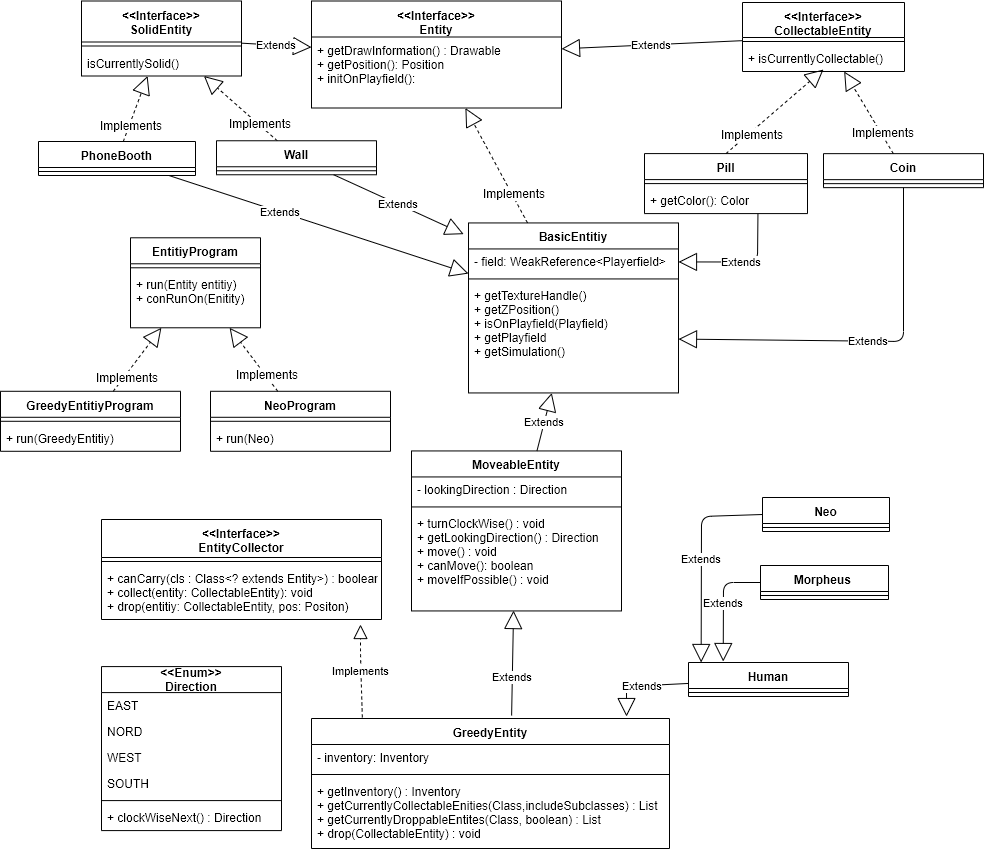
\includegraphics[width=1.2\textwidth]{figures/icge-class-diagramm.png}}

    % Aufgabe 5
    \renewcommand{\workingtimeMinutes}{5}
    \titledquestion{Exceptions – Wenn etwas schief geht}

    Öffne die Klasse zu \fbox{Task0 a)} (siehe Aufgabe davor).
    Füge nach dem \texttt{// do AB1 task 5 \& 6 here} eine neue Zeile \texttt{this.player.turnClockWise();} ein.
    Starte das Programm neu und führe \fbox{Task0 a)} aus.

    In der Simulation-Konsole sollte eine \texttt{IllegalMoveException} Exception geflogen sein.
    Eine Entity darf nicht in eine Wand reinlaufen.
    Wenn sie es dennoch versucht wird eine Exception geworfen.

    % Aufgabe 6
    \renewcommand{\workingtimeMinutes}{15}
    \titledquestion{Operationen selber aufrufen}

    Öffne die Klasse \texttt{Solution1} im Paket \solutionPackage.
    Eine Operation die Neo ausführen soll steht schon in der \texttt{solve} Operation der \texttt{Solution1} Klasse.
    Mit \texttt{this} kann man auf Daten des aktuellen Objekts zugreifen.
    In der \texttt{Solution1} Klasse bezieht sich this auf das aktuelle Objekt der \texttt{Solution1} Klasse.
    In Zeile 27 wird dem Attribut \texttt{player} das \texttt{Neo} Objekt zugewiesen.
    In Zeile 36 wird dann auf diesem \texttt{Neo} Objekt das Kommando \texttt{move()} aufgerufen.

    \begin{parts}
        \part Bewege Neo auf die Telefonzelle indem du die fehlenden Kommandos in der \texttt{solve} Operation der \texttt{Solution1} Klasse ergänzt.
        \part Aus welcher Klasse in dem Klassendiagramm weiter oben kommt das Kommando \texttt{move()}?
    \end{parts}
    \begin{solution}
    \begin{lstlisting}
        this.player.move();
        this.player.move();
        this.player.turnClockWise();
        this.player.move();
        this.player.move();
    \end{lstlisting}
    \end{solution}

% Aufgabe 7
\renewcommand{\workingtimeMinutes}{15}
\titledquestion{Objekt Orientierte Analyse}
\begin{parts}
\part Du willst einen neuen Laptop kaufen. also informierst du dich online und im Elektrofachgeschäft. Nachdem du dir verschiedene Geräte angeschaut hast bist du der Meinung das ein Thinkbook++ genau richtig ist. Also gehst du in JupiterMarkt und sprichst mit einem Verkäufer. Jedoch ist das Gerät das du willst leider ausverkauft. Weil du nicht warten möchtest bestellst du das Gerät lieber in einem Onlineshop. Du entscheidest dich für Nil.com

\begin{enumerate}
 \item[a)] Identifiziere (und schreibe auf) Klassen und Objekte die du in diesem Text finden kannst.
 \item[b)] Ist es sinnvoller JupiterMarkt und Nil.com durch die selbe Klasse zu representieren oder nicht? und warum
 \item[c)] Beschreibe 10 potenzielle Attribute für die Klasse Computer
\end{enumerate}
\part Du hast eine e-mail von deinem Team-leiter bekommen:\\
\framebox{\parbox{\columnwidth-4\fboxsep}{
Hi,
Der Cheff hat mir eine E-mail von einem Kunden weitergeleitet und gemeint wir sollen das Projekt übernehmen. Annika und Jürgen sind ja noch im Urlaub und Sven setzt schonmal ein projekt auf. Kannst du dir das Blabla vom Kunden schon mal anschauen und die Klassen und Attribute rausschreiben!

Danke und grüße
David

--ForwardedMessage.eml\\
\textbf{Subject:} Lagerhallen Rechner Sanftwahre\\
\textbf{From:} Karl-Heinz-Mueller@storage.logistik.nil.eu.de\\
\textbf{Date:} 5.10 9:37\\
\textbf{To:} auftrag@comsulting.de\\

Sehr geehrt Damen und Herren,\medskip

ich bin leiter eine Lagerhalle bei Neckars-Ulm. Das ist die Zentrale Lagerhalle von Nil.de, für Ba-Wü. Kennen sie vielleicht ist direkt beim Ortseingang.

Wie auch immer, bei uns herrscht immer ein Chaos und ich möchte endlich auf meinen Computer sehen können, was da vor sich geht. Dann muss ich nicht mehr rumlaufen, um überall meine Augen zu haben.
Wir haben uns letztes Jahr so ein Funkkarten System gekauft. Da hat jeder hier so eine EC-karte und kann die an einen Kasten bei der Tür halten um sie auf zu schließen. Leider ohne die Computer dinge, die sollen ja auch von ihnen kommen. Also jedesmal wenn ein mitarbeiter seine Karte dranhalten. Soll der beim Hauptrechner sagen wer da gerade welche tür aufmachen möchte und der Antwortet dann geht. Natürlich nur wenn ich ihm vorhergesagt habe es geht, oder mein Sicherheitsbeauftragter. Ach ja ich möchte auch das man vorher irgendwie ein Passwort eingibt. Ich hasse die dinger zwar wie die Pest aber, dann kann das nicht jeder machen. 
Und die Mitarbeiter sollen sich auch anmelden können und sehen wo sie rein dürfen und wie Lange sie gearbeitet haben. Also wie lange zwischen reingehen durch die eingangstür und rausgehen vergangen ist. Ich kann das natürlich auch sehen.\\
Desweiter scannen natürlich die mitarbeiter mit so Handgeräten alle Waren ein wenn sie reinkommen und wenn sie rausgehen.
\medskip

PS: Mein Anwalt hat gemeint, niemand darf die Arbeitszeit verändern dürfen, sondern nur Anfragen.
\medskip
Mit Freundlichen Grüßen.\\Karl-Heinz\\ M?:uller
}}
\part 
Markiere im folgenden Text alle Klassen und Objekte.

Es ist 15 Uhr und du freust dich auf deine Lieblingsshow, welche demnächst im TV auf Sender 7 läuft. 
Du läufst in die Küche, um dir Softdrinks und Snacks zu holen. Schnell merkst du jedoch, dass du beides nicht mehr vorrätig hast, und entscheidest dich, mit dem Auto zum Laden zu fahren und einzukaufen.

Du schnappst dir deine Schlüssel und deinen Geldbeutel und läufst zu deinem Auto, einem blauen Golf 5, welches auf der Straße "Jupiterweg" steht. 
Am Lidl angekommen schnappst du dir schnell eine Tüte funny-frisch Chips und zwei Flaschen Coca-Cola und rennst fast schon zu den Kassen, damit du deine Lieblingsshow nicht verpasst. Dort merkst du, dass du kein Geld dabei hast, weshalb du mit deiner Kreditkarte bezahlst. Voller Vorfreude fährst du nun nach Hause. 
\end{parts}
\end{questions}